% Chapitre de contribution n° 3 (TOP20 pick 3, id Z-UO-TIERED)
% Sources : papers/universal_optimality_tiered/ (universal_optimality_tiered.tex, gen_numbers.tex,
% publication_meta_v2.json), results/discovery/ledger/manuscript_audit_2026-10-11.md,
% papers/ar_yukawa_crystal/data/NUMERICS.md (erratum), TOP20.json.
\chapter[Le triangle, rangement le moins coûteux]{Le triangle, rangement le moins coûteux : des conséquences vérifiées et une simulation}
\reference{Publié le 11 octobre 2026.\\ v1 : doi:10.5281/\\zenodo.23293112\\ v2 : doi:10.5281/\\zenodo.23293429}

\section*{L'idée en une image}

\begin{analogie}
Posez des billes identiques à plat sur un grand plateau, une seule couche, et imaginez qu'elles se repoussent toutes
un peu, même de loin. Un théorème dit quelle disposition coûte le moins d'énergie : le motif en triangles, où chaque
bille a six voisines, comme les centres des alvéoles d'une ruche. Une simulation, elle, secoue le plateau pour voir si les billes trouvent ce motif toutes seules.

\emph{Où l'image s'arrête :} de vraies billes ne se poussent qu'au contact, sur un plateau fini ; le théorème parle
d'une répulsion à distance, sur un plan infini, à densité fixée.
\end{analogie}

\section*{Ce qui a été fait}

En septembre 2026, OpenAI a publié une preuve, produite par une IA et vérifiée par ordinateur, d'un énoncé que la
littérature décrivait comme un problème ouvert important : pour une large famille de répulsions, l'arrangement triangulaire a la plus petite énergie parmi
toutes les façons de placer des points dans le plan avec une densité donnée. Ce chapitre et les suivants appellent ce
résultat « le théorème amont ». Le travail présenté ici en tire des conséquences vérifiées par la machine, et confronte
un cas physique à une simulation.

Deux conséquences sont prouvées. D'abord, le réseau triangulaire, dilaté comme il faut, est optimal à \emph{toutes}
les densités, au sens d'une définition classique de l'« optimalité universelle » (dans une version un peu plus faible,
qui compare des moyennes au sens d'une limite inférieure). Ensuite, l'optimum n'est pas unique : si l'on retire un
seul point au réseau, ni la densité ni l'énergie ne changent, et pourtant ce réseau troué n'est pas une copie déplacée
du réseau complet.

\begin{encadre}
\textbf{À faire avec un crayon : pourquoi le réseau troué n'est pas une copie.} Un déplacement rigide (translation,
rotation, symétrie) conserve les milieux : si $M$ est le milieu de $P$ et $Q$, son image est le milieu des images.
Notez $a\approx1{,}075$ l'écart entre voisins. Dans le réseau troué, les points $(a,0)$ et $(2a,0)$ existent, et le
point « symétrique de $(2a,0)$ par rapport à $(a,0)$ » est $2(a,0)-(2a,0)=(0,0)$ : c'est le trou
(figure~\ref{fig:c03}a). Si un déplacement envoyait le réseau complet sur le réseau troué, deux points $u$ et $v$ du
réseau complet arriveraient en $(a,0)$ et $(2a,0)$. Le point $2u-v$ est encore dans le réseau complet, et il
arriverait en $(0,0)$, qui manque. Contradiction.

\textbf{Le trou ne coûte rien en moyenne.} Dans un disque de 1\,000 points, en retirer un change la moyenne par point
d'un facteur $1000/999\approx1{,}001$ ; avec un million de points, $1{,}000001$. À la limite, plus rien.
\end{encadre}

Côté physique, le travail étudie la répulsion « écrantée » (dite de Yukawa), celle de grains chargés dans un plasma
poussiéreux : elle s'affaiblit plus vite que la répulsion électrique ordinaire, avec un paramètre d'écrantage
$\kappa$. Qu'elle appartienne à la famille du théorème est ici un raisonnement humain, non vérifié par la machine
\niveau{C} (il le sera au chapitre suivant). Une simulation de 288 particules, menée avec le solveur CVODE réécrit en Rust par le
projet, laisse chaque configuration désordonnée glisser vers un minimum d'énergie. Aucune des 100 relaxations à
$\kappa=2$, ni des 50 à $\kappa=1$, n'est descendue sous l'énergie du réseau triangulaire. Le recuit simulé (on
chauffe puis on refroidit lentement) n'a trouvé le réseau parfait qu'une fois sur 20 dans chaque famille de départs à
$\kappa=2$, et a échoué au critère annoncé à $\kappa=1$.

\begin{figure}[htbp]
\centering
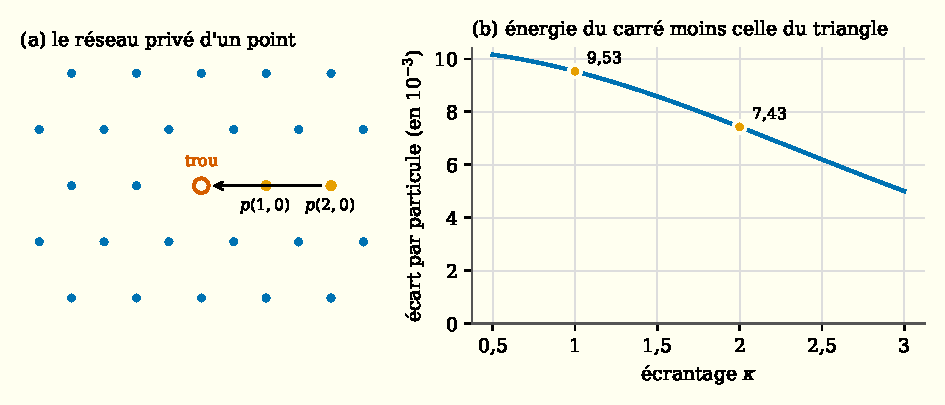
\includegraphics[width=\linewidth]{figures/c03_lacune}
\caption{(a) L'argument du trou. (b) Écart d'énergie par particule, réseau carré moins réseau triangulaire, recalculé
avec la loi exacte, sans coupure (niveau X) ; il redonne aux points marqués les valeurs exactes du chapitre suivant,
dont les valeurs publiées le 11 octobre, avec coupure, diffèrent d'au plus $2{,}2\times10^{-6}$.}
\label{fig:c03}
\end{figure}

\section*{Comment on s'est assuré que ce n'est pas faux}

\niveau{A} \emph{Le juge a regardé.} Les deux conséquences sont des théorèmes Lean (Lean est un programme qui contrôle
chaque pas logique d'une preuve). Ils n'utilisent que les trois hypothèses de base admises partout, deux pièges
volontaires (une preuve laissée en blanc, un axiome inventé) ont été détectés, et le module a été rejoué sans erreur
par un second programme de contrôle le 26 octobre 2026. La simulation reste \niveau{X} : elle guide, elle ne prouve
rien.

Chaque affirmation est rangée dans un registre de 22 lignes avec son niveau de confiance. Ce registre refuse de
donner son feu vert : 6 lignes de niveau A attendent encore qu'une personne vérifie que l'énoncé dit bien ce qu'on
croit. L'auteur a choisi de publier avec ces drapeaux visibles et l'a écrit dans l'article. Un audit indépendant par
un autre agent d'IA a demandé trois corrections de texte, faites, puis une seconde relecture a suivi. Ce résultat,
comme tout le livre, a été produit et audité par des agents d'IA ; aucun humain spécialiste ne l'a relu, et le
théorème amont lui-même n'a pas encore été évalué par des pairs. Dans la simulation, les témoins se sont comportés
comme prévu : un réseau parfait reste en place, un réseau carré se révèle instable (72 directions où l'énergie
descend), et une boîte qui ne peut pas contenir de triangles parfaits garde ses défauts.

\section*{Ce que ça ne dit pas}

\begin{limite}
\begin{itemize}
\item Tout repose sur le théorème amont, produit par une IA et non encore relu par des pairs.
\item La simulation coupait la force au-delà d'une distance 8. Cette coupure abaissait l'énergie d'environ $0{,}018$ à
$\kappa=1$, plus que l'écart carré--triangle (environ $0{,}0095$) : un erratum, corrigé au chapitre suivant.
\item L'échec du recuit à $\kappa=1$ montre la faiblesse de l'outil, pas un défaut du théorème.
\item L'unicité parmi les arrangements périodiques n'est ni affirmée ni étudiée.
\end{itemize}
\end{limite}

\section*{Pour aller plus loin}

Ce travail sert de gabarit à toute la suite : l'IA propose, le calcul explore, Lean juge, l'humain décide de publier.
La version 2 ajoute des figures et des protocoles de laboratoire. Article : doi:10.5281/zenodo.23293429.
